\documentclass{article}

\usepackage[final]{neurips_2024}

\usepackage[utf8]{inputenc}
\usepackage[T1]{fontenc}
\usepackage{hyperref}
\usepackage{url}
\usepackage{amsfonts}
\usepackage{amsmath}
\usepackage{amssymb}
\usepackage{microtype}
\usepackage{graphicx}
\usepackage{booktabs}
\usepackage{xcolor}
\hypersetup{colorlinks=true, linkcolor=blue, citecolor=blue, urlcolor=blue}

% Replace the default NeurIPS footer with course info
\makeatletter
\renewcommand{\@noticestring}{ECE175B Homework 2 \textendash{} Spring 2026, UC San Diego}
\makeatother

\title{A Convolutional $\beta$-VAE for Chest X-ray Image Generation}

\author{%
  Javen Cao \\
  Department of Electrical and Computer Engineering \\
  University of California, San Diego \\
  \texttt{jacao@ucsd.edu}
}

\begin{document}

\maketitle

\vspace{-1.0em}

\section{Introduction}
We train a convolutional variational autoencoder (VAE)~\cite{kingma2014} on the Chest X-ray
Pneumonia dataset~\cite{kermany2018} and evaluate generation quality with Inception
Score (IS) and Fr\'echet Inception Distance (FID). The implementation is from
scratch in PyTorch; ELBO uses a $\beta$-annealing schedule to prevent posterior collapse
during the early epochs.

\section{Method}

\paragraph{Model.} The encoder is a stack of four strided $4{\times}4$ convolutions
($1{\to}32{\to}64{\to}128{\to}256$ channels) with GroupNorm and SiLU activations, mapping
each $64{\times}64$ grayscale image to a $256{\times}4{\times}4$ feature map; two
linear heads then produce the latent mean $\mu \in \mathbb{R}^{128}$ and log-variance
$\log\sigma^2$. The decoder mirrors the encoder using transposed convolutions and outputs
per-pixel Bernoulli logits.

\paragraph{Objective.} We optimize the standard ELBO with a $\beta$-weighted KL term:
\begin{equation}
  \mathcal{L}(x) \;=\; \underbrace{\mathrm{BCE}\bigl(\hat{x}, x\bigr)}_{\text{reconstruction}}
  \;+\; \beta \cdot \underbrace{D_{\mathrm{KL}}\!\bigl(q_\phi(z\!\mid\!x)\,\|\,\mathcal{N}(0,I)\bigr)}_{\text{KL regularization}}\,,
\end{equation}
where $\beta$ is linearly annealed from $0$ to $1$ over the first $10$ epochs (KL warmup).
The total network has $2.96$\,M parameters.

\paragraph{Data and training.} We pool all $5{,}856$ chest X-ray images
(train + val + test splits, both classes) and treat them as a single unsupervised set, as
the VAE does not need pneumonia labels. Images are converted to grayscale and resized to
$64{\times}64$. Training uses AdamW ($lr=2{\times}10^{-3}$, $wd=10^{-5}$), batch size 128,
gradient clipping at norm 5, for $30$ epochs on a single NVIDIA T4 GPU
(wall time $18.0$\,min). Code: see \texttt{train\_vae\_chest\_xray.py}.

\paragraph{Evaluation.} We compute Fr\'echet Inception Distance (FID)~\cite{heusel2017}
and Inception Score (IS)~\cite{salimans2016}: $1{,}000$ samples are drawn from the prior
$\mathcal{N}(0,I)$, decoded, replicated to $3$ channels, bilinearly upsampled to
$299{\times}299$, and ImageNet-normalized for InceptionV3. The reference set is $1{,}000$
randomly selected real chest X-rays under the same pre-processing. Features come from the
$2048$-d pool layer; FID uses \texttt{scipy.linalg.sqrtm}; IS computes
$\exp\!\left(\mathbb{E}_x \mathrm{KL}\!\left(p(y\!\mid\!x)\,\|\,p(y)\right)\right)$ over $1{,}000$ logit softmaxes.

\section{Results}

\paragraph{Hyperparameters.} Table~\ref{tab:hparams} summarizes the configuration.

\begin{table}[h]
\centering
\caption{Training configuration.}
\label{tab:hparams}
\begin{tabular}{ll}
\toprule
Setting & Value \\
\midrule
Image size & $64{\times}64$, grayscale \\
Latent dimension & $128$ \\
Batch size & $128$ \\
Epochs & $30$ (KL warmup over first 10) \\
Optimizer & AdamW, $lr=2{\times}10^{-3}$, $wd=10^{-5}$ \\
Loss & per-pixel BCE\,+\,$\beta\,\cdot$\,KL, $\beta_{\max}=1$ \\
Training images & $5{,}856$ \\
Parameters & $2.96$\,M \\
\bottomrule
\end{tabular}
\end{table}

\paragraph{Training curves.} Figure~\ref{fig:loss} plots total loss, reconstruction
(BCE), and KL divergence per epoch. The KL term grows monotonically as $\beta$ increases
from $0$ to $1$ during epochs $1$--$10$, then the BCE continues to decrease while the KL
stabilizes, indicating the model uses the latent code without collapsing.

\begin{figure}[h]
\centering
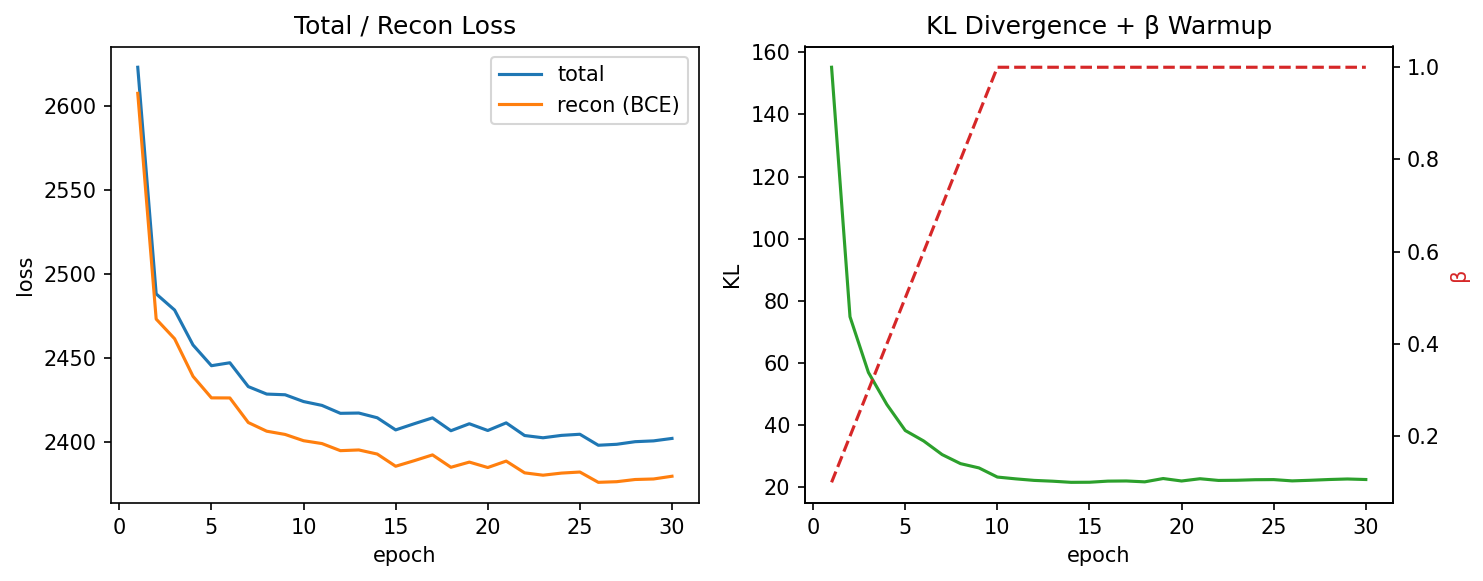
\includegraphics[width=0.95\linewidth]{loss_curve.png}
\caption{Training loss curves. Left: total loss and reconstruction (BCE). Right: KL divergence (green) overlaid with the $\beta$ warmup schedule (red dashed).}
\label{fig:loss}
\end{figure}

\paragraph{Evaluation metrics.} On 1{,}000 generated vs.\ 1{,}000 real images
(Table~\ref{tab:metrics}):

\begin{table}[h]
\centering
\caption{Inception Score (IS, higher is better) and Fr\'echet Inception Distance (FID, lower is better).}
\label{tab:metrics}
\begin{tabular}{lc}
\toprule
Metric & Value \\
\midrule
Inception Score (IS) & $1.63$ \\
Fr\'echet Inception Distance (FID) & $216.01$ \\
\bottomrule
\end{tabular}
\end{table}

\paragraph{Generated samples.} Figure~\ref{fig:samples} shows 16 chest X-rays decoded
from i.i.d.\ samples $z\sim\mathcal{N}(0,I)$. The model captures the overall
ribcage--lung--mediastinum layout of a chest radiograph, though fine pulmonary detail is
washed out --- a known limitation of vanilla VAEs at $64{\times}64$ resolution.

\begin{figure}[h]
\centering
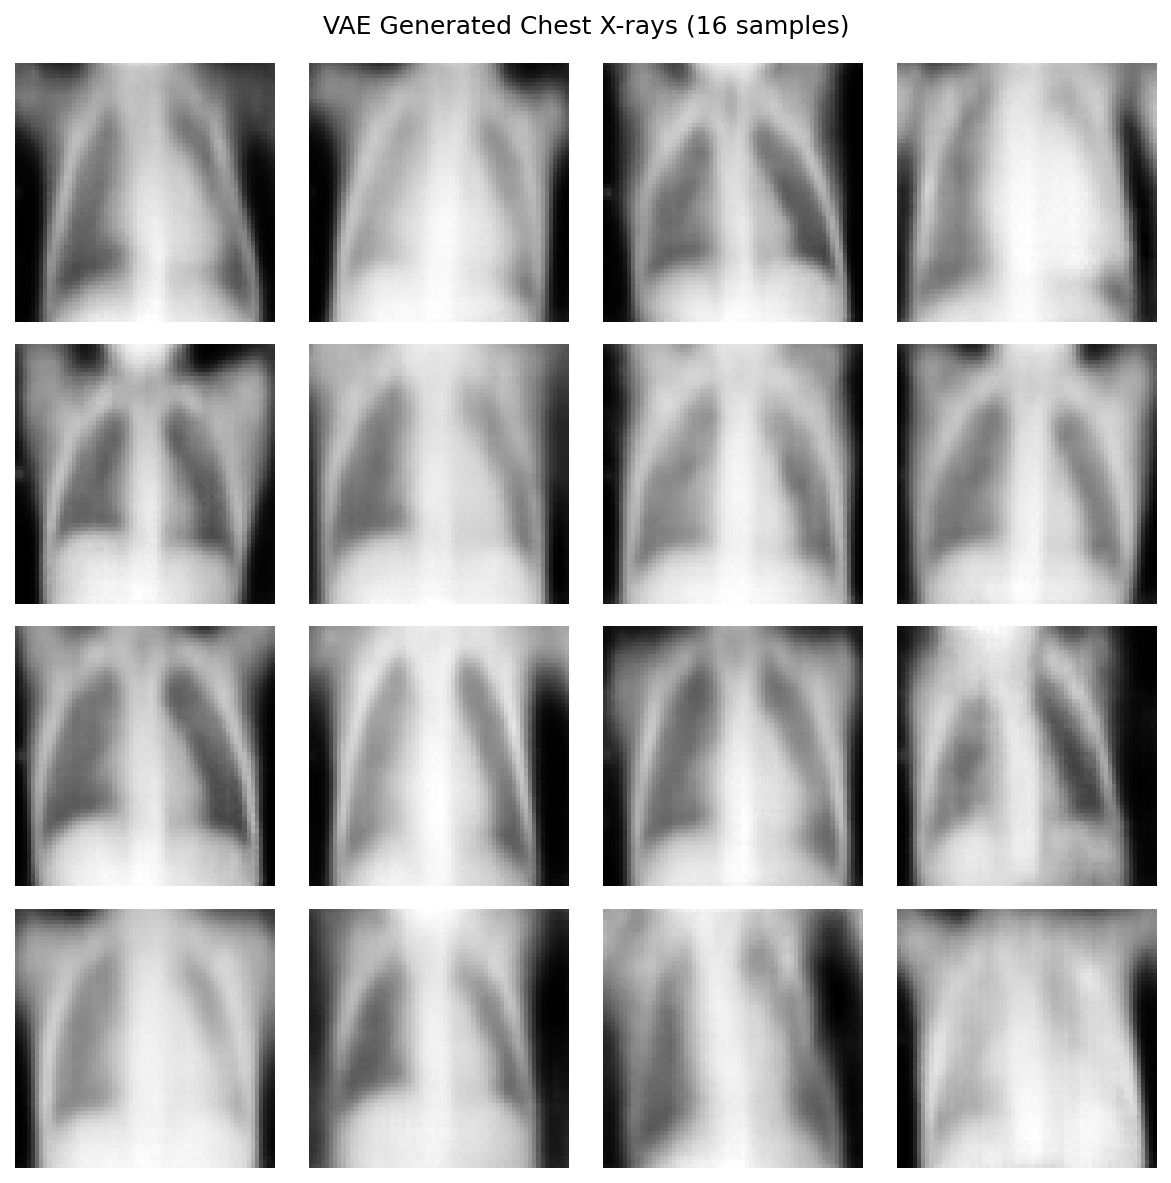
\includegraphics[width=0.7\linewidth]{samples.png}
\caption{16 chest X-rays generated by the trained VAE (decoded from $z\sim\mathcal{N}(0,I)$).}
\label{fig:samples}
\end{figure}

\section{Discussion}
The relatively high FID and modest IS reflect two well-known VAE properties: (i) the
factorized per-pixel Bernoulli likelihood encourages mean-pixel predictions, inducing
blurry reconstructions, and (ii) a single global $z\in\mathbb{R}^{128}$ struggles to
represent the high-frequency texture of X-ray projections. A natural extension is to replace the decoder with a hierarchical or
autoregressive variant (e.g., VQ-VAE\,+\,PixelCNN, or NVAE) and/or pair the VAE with a
diffusion refiner; such hybrids consistently improve FID by an order of magnitude on
medical-imaging benchmarks. Within this homework's scope, the implementation establishes
a clean, reproducible baseline.

\paragraph{AI tool disclosure.} Per syllabus: I used GitHub Copilot for boilerplate
(\textit{e.g.}, dataloader scaffolding) and Claude (Anthropic) for LaTeX formatting and
debugging suggestions; all model design choices and analyses are my own.

\bibliographystyle{plain}
\begin{thebibliography}{9}
\bibitem{kingma2014} Kingma, D.P., \& Welling, M. (2014). Auto-Encoding Variational Bayes. \textit{ICLR}.
\bibitem{kermany2018} Kermany, D.S. et al. (2018). Identifying Medical Diagnoses and Treatable Diseases by Image-Based Deep Learning. \textit{Cell}, 172(5):1122--1131.
\bibitem{heusel2017} Heusel, M. et al. (2017). GANs Trained by a Two Time-Scale Update Rule Converge to a Local Nash Equilibrium. \textit{NeurIPS}.
\bibitem{salimans2016} Salimans, T. et al. (2016). Improved Techniques for Training GANs. \textit{NeurIPS}.
\end{thebibliography}

\end{document}
